\section{State Of The Art Analysis}\label{sec:state-of-the-art-analysis}
This section will discuss the state of the art of technologies already used in amusement parks around the world.
It will also focus on those used, or that have been used in the past, in the park Mirabilandia in Italy.

Firstly, since an incarnation of a Micro City as an amusement park has the crucial ``queue'' concept, we searched for ``smart''
and innovative solutions to manage that.
Another important point in a Micro City is that the system should be able to send notifications based on the location of
the people at a certain time.
Another is the personalization of the experience.
Events???

\subsection{Virtual Queueing}\label{subsec:virtual-queueing}
What is.

Also why: Virtual queuing helps remove the number one frustration of guests (waiting in lines), increasing guest
satisfaction and revenue.
Virtual queuing can add new revenue streams to your organization, and it can also unlock
secondary spending as guests visit F&B locations or retail locations.
(https://www.accesso.com/learn/virtual-queuing-less-waiting-more-fun)

Also other uses of the virtual queueing (Boston Airport etc.)
\subsubsection{Accesso's Virtual Queueing}
Their technology is patented.

\subsubsection{Accesso Technology Group Virtual Queueing Products}
Accesso Technology Group\footnote{\url{https://www.accesso.com/}} (formerly Lo-Q) is an English company that provides
devices and mobile apps for virtual queueing to several clients, including theme parks like the ``Six Flags'' corporation in the US
and ``LEGOLAND Windsor Resort'' in the UK\@.

Their products for virtual queueing are \textit{Qsmart} and \textit{Prism}\footnote{\url{https://www.accesso.com/solutions/virtual-queuing/prism}}
and they also used to sell the devices \textit{Qbot} and \textit{Qband} no longer available to this days~\cite{accesso-wikipedia}.
With Qsmart people can access the virtual queueing services directly from their smartphones whereas Prism is a ``smartwatch-like''
wearable.

The latter is a standalone device, with no need for kiosks or charging stations to support its use.
Also, is waterproof, hypoallergenic, durable and brandable~\cite{prism-desc}.
As can be observed in Figure~\ref{fig:prism}, Prism provides the following functionalities:
\begin{itemize}
    \item Virtual queueing: \textit{visitors} can manage their reservation in line and monitor the line status
    \item Payments: \textit{visitors} can make payments thanks to a secure NFC technology
    \item Messaging: \textit{visitors} can receive push notifications for proximity-based marketing (i.e.\ trigger nearby events based on people location, Figure~\ref{fig:prism-icecream}), operational updates, or the status of pending virtual queue positions
    \item Photography: Prism allows automated tagging of ride and park photographs
    \item Access: \textit{visitors} can easily access park turnstiles, guest lockers, resort hotel rooms, etc.
    \item Intelligence: Prism collects real-time information about the users' behaviour during the visit for marketing and park operations purposes
\end{itemize}

\begin{figure}[H]
    \centering
    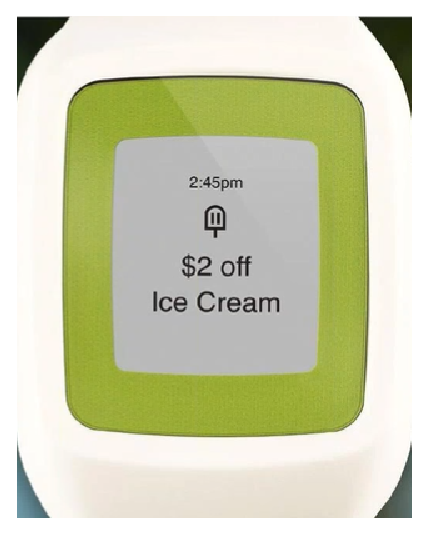
\includegraphics[width=0.3\textwidth]{img/prism-icecream}
    \caption{Example of a push notification based on the visitor proximity to an ice cream shop}
    \label{fig:prism-icecream}
\end{figure}

In addition to their patented virtual queueing technologies, Prism works on a \textbf{proprietary network} and uses three ways to communicate:
\begin{itemize}
    \item \textbf{Bluetooth Low Energy (BLE Beacon):} allows sending real-time messages to \textit{visitors} based on their location, triggers interactions and gain valuable insights about visitors' flow throughout the park
    \item \textbf{Near Field Communication (NFC):} used for access, payments, rentals, etc.
    \item \textbf{Long Range Sub-GHz Two-Way Radio:} allows \textit{visitors} to reserve and modify queueing reservations without having to use their smartphone from where they are
\end{itemize}

Finally, the wearable technical specifications consist of a Toughened Glass Lens with Touch Screen, a Reinforced Housing, a 32mm High Resolution 168 x 144 LCD Display, a Rubber O‑Ring Seal Waterproof to 20m / 65ft,
a Vibration Notification Motor and a CR3032 Coin Cell supporting over 200 days of park usage.

\begin{figure}[H]
    \centering
    \begin{subfigure}[b]{0.85\textwidth}
        \centering
        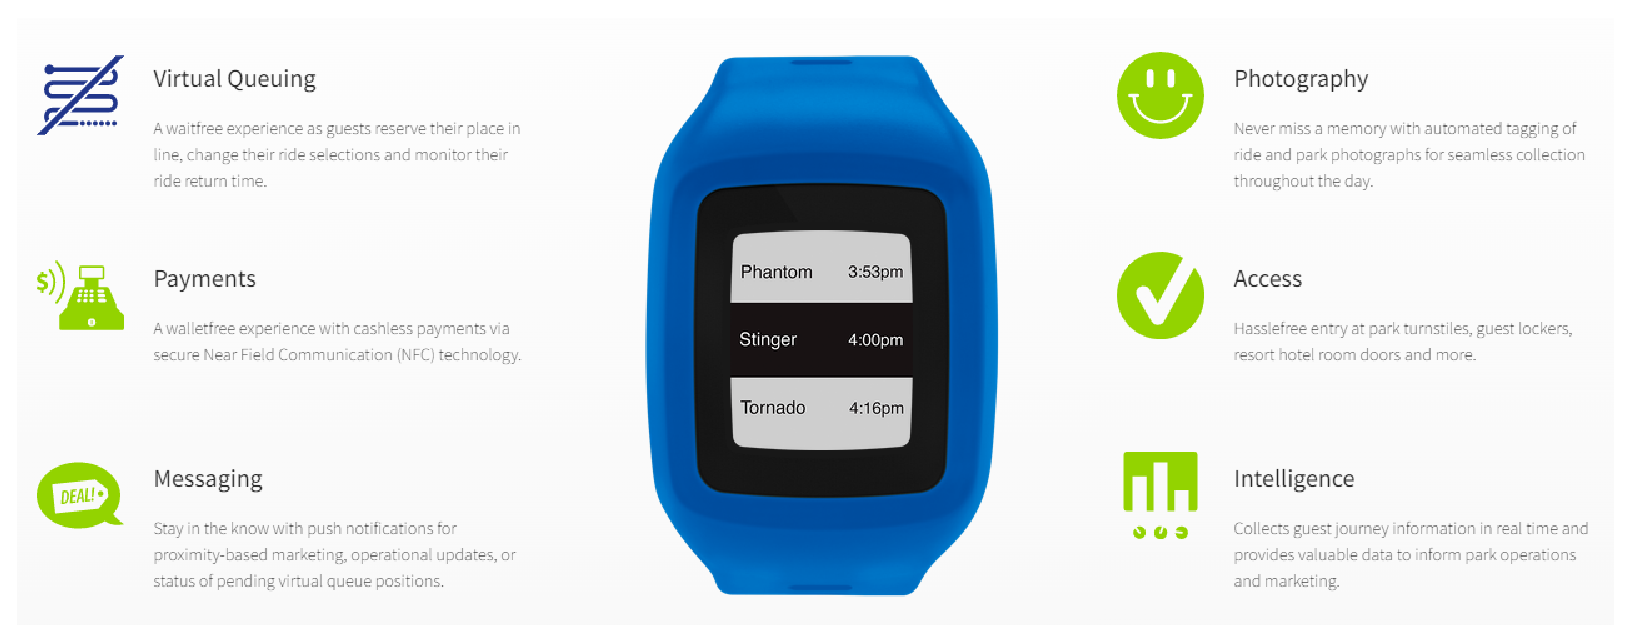
\includegraphics[width=\textwidth]{img/prism}
        \caption{Prism main functionalities}
        \label{fig:prism}
    \end{subfigure}
    \hfill
    \begin{subfigure}[b]{0.85\textwidth}
        \centering
        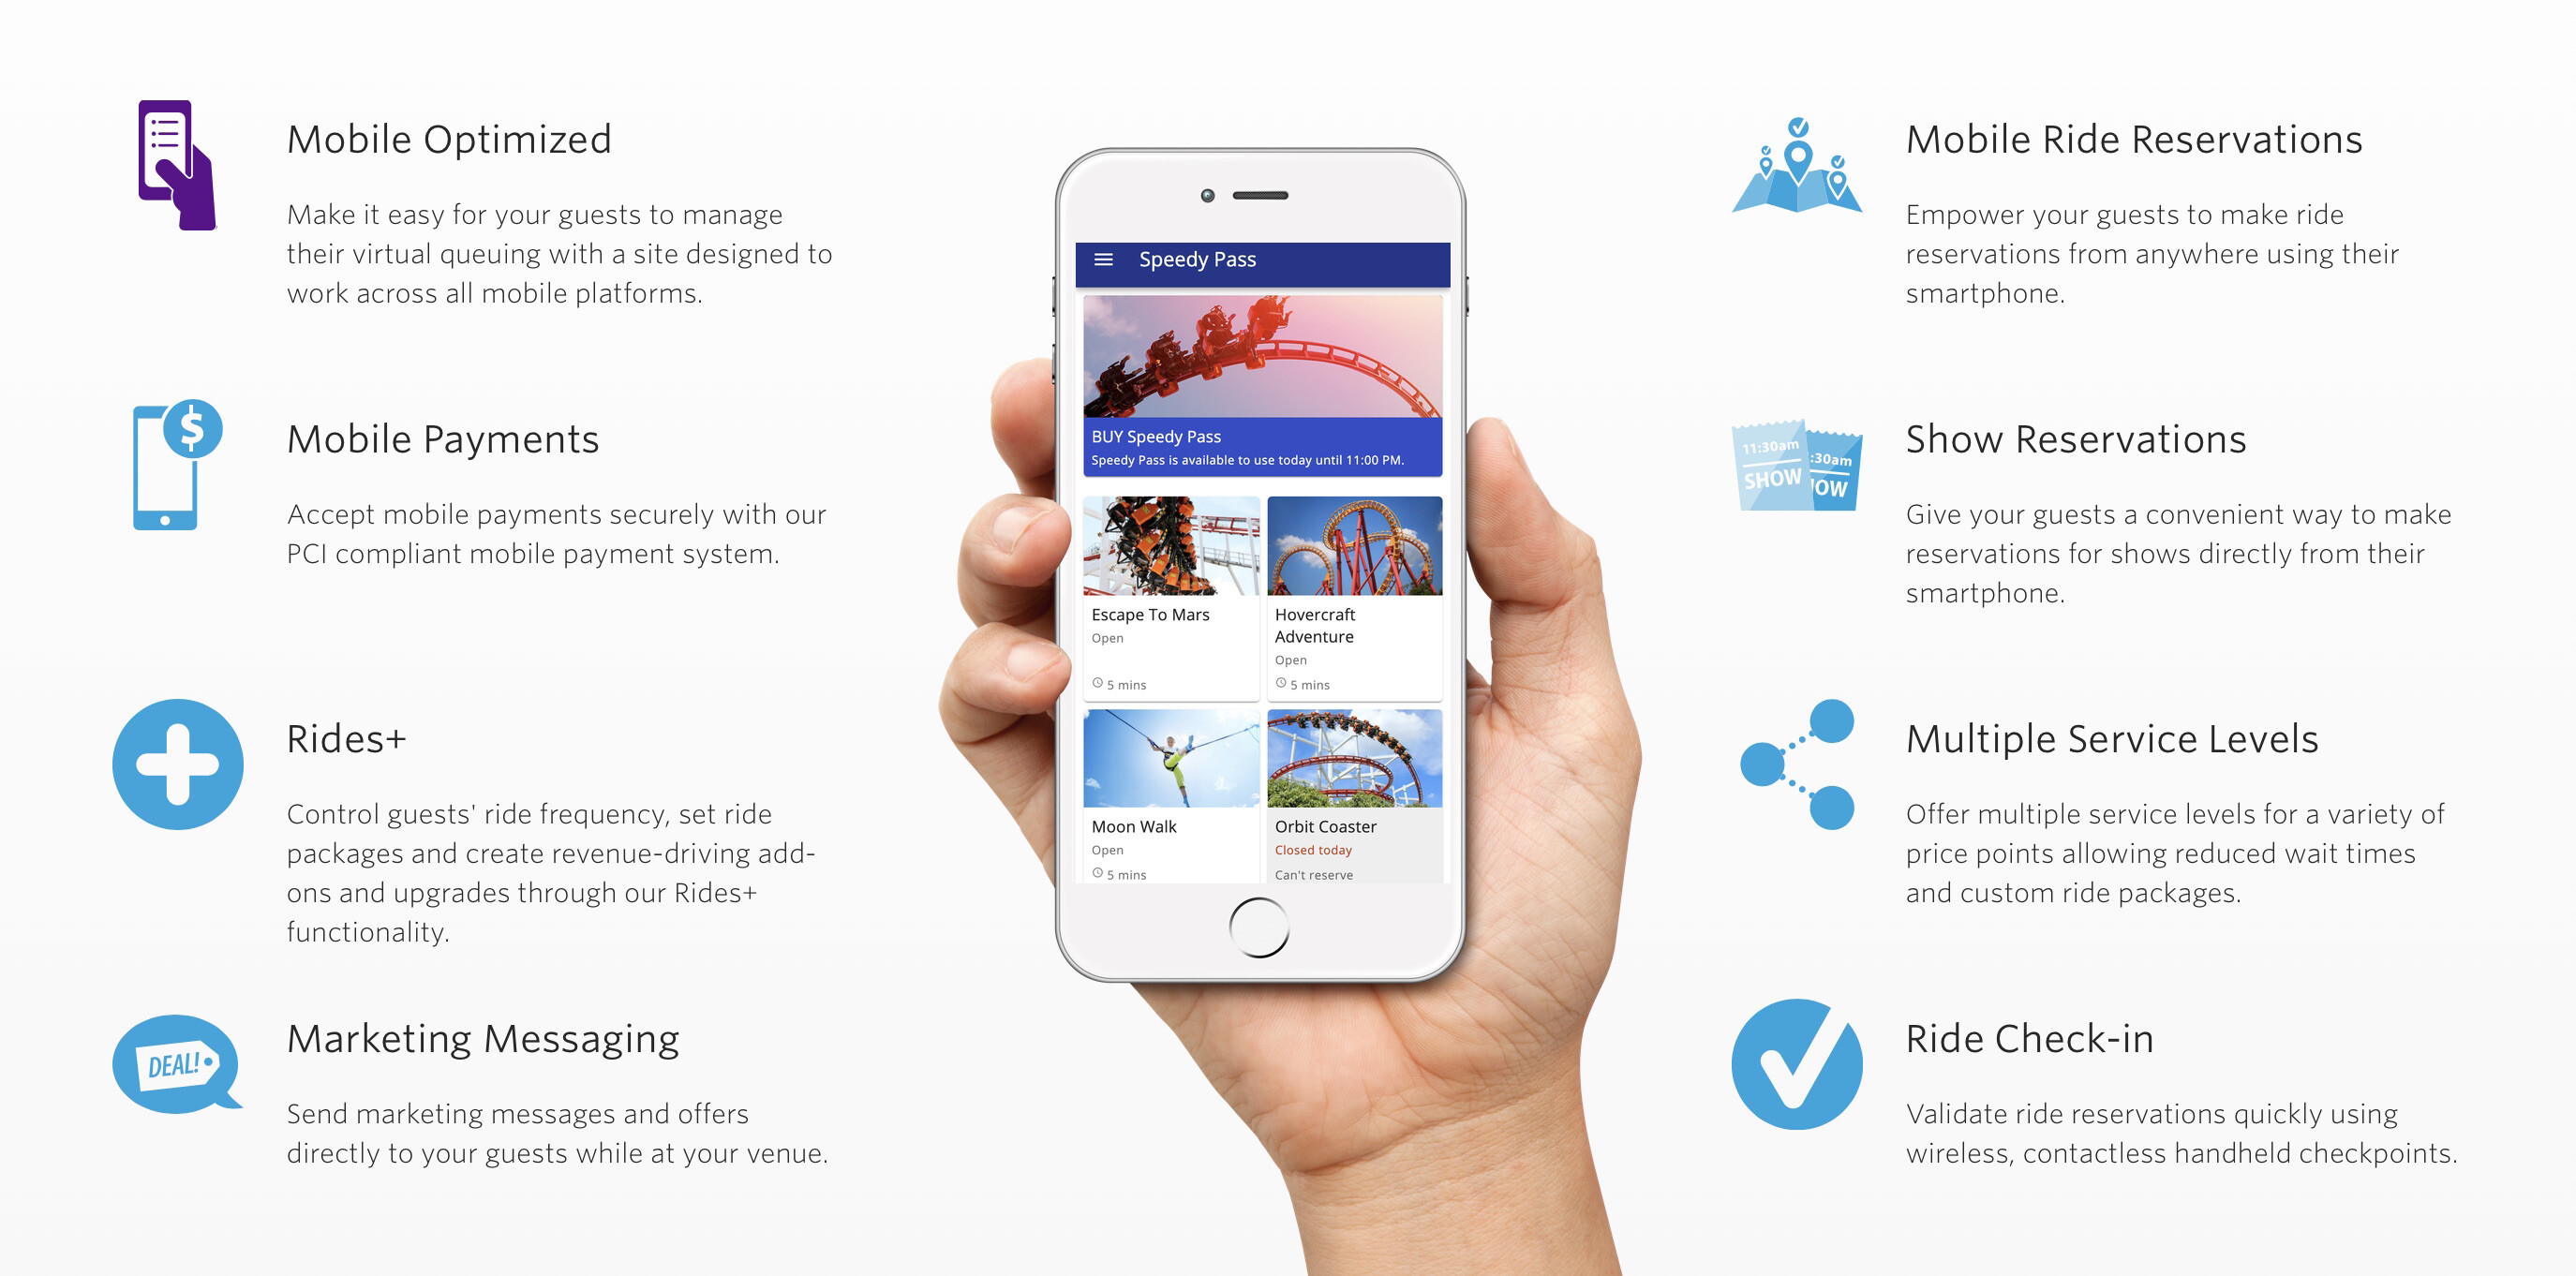
\includegraphics[width=\textwidth]{img/qsmart}
        \caption{Qsmart main functionalities}
        \label{fig:qsmart}
    \end{subfigure}
    \caption{Accesso's products for virtual queueing\footnotemark}
    \label{fig:prismart}
\end{figure}
\footnotetext{\url{https://www.accesso.com/solutions/virtual-queuing}}

On the other hand, QSmart is a ready-to-use platform and utilizes the visitor's smartphone hardware, is cloud based
and operates via Wi-Fi.

The application allows \textit{visitors} to easily make ride and show ticket purchases as well as shows
live wait times and accepts mobile payments.
It can also be integrated with other Accesso's products like, for instance, an online ticketing system.



Both Prism and QSmart interact with the Virtual Queue Management System, where customers can consult
analytics and performance data as well as control in real-time the virtual queueing solution.
However, there isn't much information about this product on the company website.

They provided their Q-Bot device also to Mirabilandia in 2009 but is no longer used to these days.


\subsection{Mirabilandia App}\label{subsec:mirabilandia-app}
- fornisce già percorsi specifici per chi è interessato a giochi adrenalinici, per bambini ecc.

\subsection{Mirabilandia - V Pass}\label{subsec:mirabilandia-v-pass}
differenza V Pass e Flash Pass.
il Disney FastPass

\subsection{Legoland Windsor - Reserve and Ride}\label{subsec:legoland-windsor---reserve-and-ride}
